% $Id: Attribute_obj.tex,v 1.4.2.4 2010/02/01 20:49:37 svasquez Exp $
%
% Earth System Modeling Framework
% Copyright 2002-2010, University Corporation for Atmospheric Research,
% Massachusetts Institute of Technology, Geophysical Fluid Dynamics
% Laboratory, University of Michigan, National Centers for Environmental
% Prediction, Los Alamos National Laboratory, Argonne National Laboratory,
% NASA Goddard Space Flight Center.
% Licensed under the University of Illinois-NCSA License.


The following is a simplified UML diagram showing the structure of the
Attribute class.  See Appendix A, {\it A Brief Introduction to UML},
for a translation table that lists the symbols in the diagram and their 
meaning.

%\begin{center}
%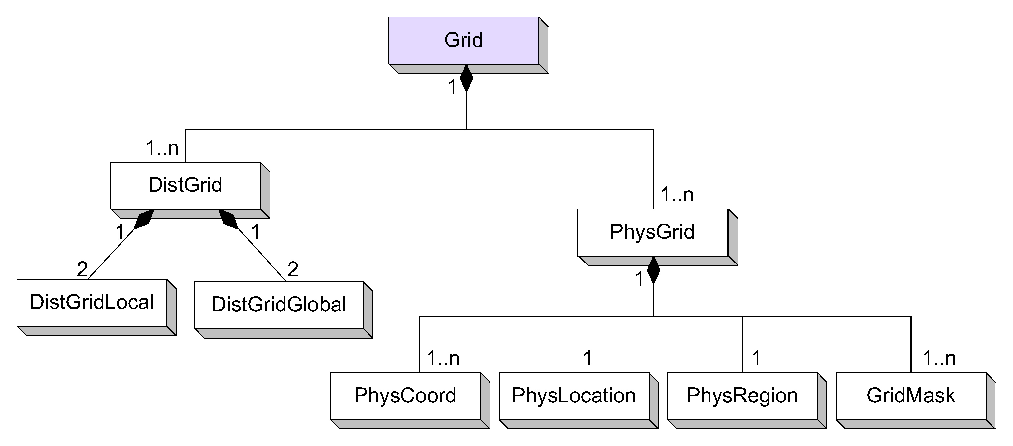
\includegraphics{Grid_obj}   
%\end{center}

Each Attribute contains a name value pair in which the value can be any of several numeric, character, and logical types.  The allowable ESMF Attribute value types include:

\begin{itemize}
\item {\tt ESMF\_TYPEKIND\_I4}
\item {\tt ESMF\_TYPEKIND\_I4} list
\item {\tt ESMF\_TYPEKIND\_I8}
\item {\tt ESMF\_TYPEKIND\_I8} list
\item {\tt ESMF\_TYPEKIND\_R4}
\item {\tt ESMF\_TYPEKIND\_R4} list
\item {\tt ESMF\_TYPEKIND\_R8}
\item {\tt ESMF\_TYPEKIND\_R8} list
\item {\tt ESMF\_TYPEKIND\_Logical}
\item {\tt ESMF\_TYPEKIND\_Logical} list
\item {\tt EMSF\_TYPEKIND\_Character}
\end{itemize}

All Attributes also contain character strings specifying the convention, type, and object of the Attribute for the purpose of keeping track of attribute packages.  All Attributes contain a pointer to a list of pointers to other Attributes, which is initialized as {\tt ESMF\_NULL} until specified otherwise.
